% !TEX root = ./../main.tex
\chapter{Introduction to Molecular Dynamics}
For macroscopic bodies, the motion of a system in time and space is governed by the classical equations of motion, say the Newton’s law, while reducing time and space scales, quantum mechanics kicks in. Despite the latter statement, classical laws of motion have proved to be a good approximation also at the molecular level, as long as atoms are massive enough.

In order to predict the time evolution of a complete system, such as the biomolecular system we will treat in this thesis, Newton’s equations of motion need to be integrated numerically. The necessity of a numerical integration arises from the complexity of the interactions involved in realistic systems, often nonlinear functions of positions and momenta of the particles making up the system, which makes it impossible to obtain an analytical solution for the equations of motion.

In the first part of this Chapter the laws of Classical and Statistical mechanics will be briefly summarized.
Then we will introduce the computational \acf{MD} method and analyze the main aspects of this technique.
Following some details about how the system under study is modeled are given: the \textit{empirical Force--Field} (\acs{FF}). This includes the way to consider and treat the inter--particle interactions at the \ac{MD} level with some methods to increase the computational efficiency such as the \textit{cut--off} methods for the so called \textit{short range} interactions and the \ac{PME} technique for treatment of the \textit{long range} interactions.
Then \martini \ac{FF}, the main \ac{FF} used in this thesis work, are summarized. Lastly some advanced sampling techniques are introduced: the \textit{Umbrella Sampling} and \textit{Metadynamics}. Some parts of this introductory Chapter are based on the books of Tuckerman \cite{Tuckerman}, Leach \cite{Leach}, Frenkel and Smit \cite{Frenkel} and Allen and Tildesley \cite{Allen} to which the reader is addressed for a more complete discussion.

\section{Review of classical mechanics}
The classical behavior of a system of $N$ particles with mass $m_i$ and coordinates $\vec r_1,\cdots,\vec r_N$ is described by the Newton's second law. Each particle in the system will experience a total force $\vec F_i$ and the so that second law for particle $i$ reads
\begin{equation}
	m_i \ddot{\vec{r}}_i = \vec F_i(\vec r_1,\cdots,\vec r_N)
	\label{eq:newtonLaw}
\end{equation}

The total force is defined as
\begin{equation*}
	\vec F_i(\vec r_1,\cdots,\vec r_N) = \vec{f}_i^{\ (e)}(\vec r_i) + \sum_{i\ne j}^N \vec{f}_{ij}^{\ (i)}(\vec r_i - \vec r_j )
\end{equation*}
where $\vec{f}_i^{\ (e)}$ is an external force acting on particle $i$ and $\vec{f}_{ij}^{\ (i)}$, which in general
depends only on distance between particle $i$ and $j$, is the inter-particle force that $i$ exerts on $j$ and
\textit{vice-versa}.Equations~\eqref{eq:newtonLaw} are refereed to as \textit{the equations of motion} of the
system; integrating them, with the sets of the \textit{initial conditions} at start time $t_0$ $\vec r_1(t_0),\cdots,\vec r_N(t_0)$ and $\dot{\vec{r}}_1(t_0),\cdots,\dot{\vec{r}}_N(t_0)$, the positions and the
velocities of all the particles in the system at any time are known.

Another way to write the equations of motion is to use particles momenta $\vec p_i = m_i \dot{\vec{r}}_i$ and then
the equations~\eqref{eq:newtonLaw} become
\begin{equation}
	\frac{d\vec p_i}{dt} = \vec F_i(\vec r_1,\cdots,\vec r_N)
	\label{eq:newtonLawMom}
\end{equation}
The full set of $6N$ functions $\{\vec r_1(t),\cdots,\vec r_N(t),\vec p_1(t),\cdots,\vec p_N\}$ gives us a full
description of the dynamics of the $N$--particle system. The set of functions above can be arranged in an ordered $6N$--dimensional vector
\begin{equation}
	\vec x_t = (\vec r_1(t),\cdots,\vec r_N(t),\vec p_1(t),\cdots,\vec p_N)
	\label{eq:phSpaceVector}
\end{equation}
called \textit{phase space vector} or the \textit{microstate} of the system at a time $t$. All the possible
microstates of a system generate a $6N$--dimensional space called \textit{phase space} of the system, indicated with $\Omega$. Thus $\vec x_t$ describes a particular trajectory in the phase space, i.e. the system evolution is the
motion of a phase space point.

Let us suppose that all the forces acting on the $N$--particle system are conservative; this means that it must
exist a scalar function $U = U(\vec r_1, \cdots, \vec r_N)$ called \ac{PEF}, so that
\begin{equation}
	\vec F_i(\vec r_1, \cdots, \vec r_N) = -\partial r_{i\alpha}U(\vec r_1, \cdots, \vec r_N)\ \hat e_\alpha = -\vec\nabla_i U(\vec r_1, \cdots, \vec r_N)
	\label{eq:pefForces}
\end{equation}
thus we have only to know the \ac{PEF} of the system at any time and the initial conditions to solve Newton's Law.

The kinetic energy of the system is defined as
\begin{equation}
	K(\dot{\vec r}_1,\cdots,\dot{\vec r}_N) = \sum_{i=0}^N\frac{1}{2}m_i\vec r_i \cdot \vec r_i
	\label{eq:kinetic}
\end{equation}

Supposing the system to be conservative, using the \ac{PEF} and the kinetic energy, we can define a scalar
function, called \textit{Lagrangian} of the system
\begin{equation}
	\mathcal{L}(\vec r_1, \cdots, \vec r_N, \dot{\vec r}_1,\cdots,\dot{\vec r}_N) = K(\dot{\vec r}_1,\cdots,\dot{\vec r}_N) - U(\vec r_1, \cdots, \vec r_N)
	\label{eq:lagrangian}
\end{equation}
such that
\begin{equation}
	\frac{d}{dt}\left ( \frac{\partial \mathcal{L}}{\partial \dot r_{i\alpha}}\right ) - \frac{\partial\mathcal{L}}{\partial r_{i\alpha}}
	\label{eq:EulerLagrange}
\end{equation}
This is a set of $3N$ equations where for each $i$, $\alpha=1,2,3$. These equations are called
\textit{Euler--Lagrange equations of motion}. It is easy to show that substituting the definition of $\mathcal{L}$
we obtain the Newton's second law. The Euler--Lagrange equations are a sort of generator of the equations of motion.

Using the definition of $\mathcal{L}$ \eqref{eq:lagrangian} we have
\begin{equation}
	p_{i\alpha} = \frac{\partial\mathcal{L}}{\partial \dot{\vec r}_{i\alpha}} = m_i\dot{\vec r}_{i\alpha}
	\label{eq:momentaLagrangian}
\end{equation}
thus we can express particles velocities as a function of particles momenta. Equations~\eqref{eq:kinetic}
and~\eqref{eq:momentaLagrangian} let us to express the kinetic energy in the form
\begin{equation}
	K = \sum_{i=0}^N \frac{\vec p_i \cdot \vec p_i}{2m_i}
	\label{eq:kineticP}
\end{equation}

To describe the system we can define another scalar function, called \textit{Hamiltonian} of the system
\begin{align*}
	\mathcal{H}(\vec r_1,\cdots,\vec r_N, \vec p_1, \cdots, \vec p_N) = &\sum_{i=0}^N \vec p_i \cdot \dot{\vec r}_i(\vec p_i) + \nonumber \\
	&-\mathcal{L}(\vec r_1, \cdots, \vec r_N, \dot{\vec r}_1(\vec p_1),\cdots,\dot{\vec r}_N(\vec p_N))
\end{align*}
Substituting~\eqref{eq:lagrangian} and using~\eqref{eq:kineticP} the Hamiltonian of the system is nothing that
\begin{equation}
	\mathcal{H}(\vec r_1,\cdots,\vec r_N, \vec p_1, \cdots, \vec p_N) = K(\vec p_1, \cdots, \vec p_N) + U(\vec r_1,\cdots,\vec r_N)
	\label{eq:hamiltonian}
\end{equation}
or \textit{the total energy of the system}. To obtain the equations of motion we have to solve \textit{Hamilton's equations}
\begin{equation}
	\begin{aligned}
		\dot r_{i\alpha} &=& &\frac{\partial\mathcal{H}}{\partial p_{i\alpha}} \\
		\dot p_{i\alpha} &=&-&\frac{\partial\mathcal{H}}{\partial r_{i\alpha}}
	\end{aligned}
	\label{eq:eqhamilton}
\end{equation}
Describing the system with the Hamiltonian formalism, in some cases, is more useful than Lagrangian one, first of
all because the Hamiltonian of a system is directly related to a well know physical quantity, the total energy.

\section{Review of statistical mechanics}
Using the picture of the classical mechanics described above we have a good and sophisticated machinery that allows us, knowing some information about the system in exame, i.e. initial positions and velocities of all particles and their interactions, to completely solve the equations of motion in order to get the dynamics of the system at every time. So classical mechanics encodes all the information about the \textit{microscopic} view of a system and, in principle, we can extract all the information we want about the \textit{macroscopic} proprieties of such system.
The main task of this process is to obtain the thermodynamics proprieties of a system (temperature, pressure and so on) from the complete sets of positions and velocities of all particles and thus it is necessary to have a link between microscopic and macroscopic world. In principle this can be done, but if we consider a real system we should solve a set of $6N$ equations where $N$ is of the order of the Avogadro number ($\mathcal{N}_A = 6.022 \cdot 10^{23}~\text{mol}^{-1}$); we can not think of solving such a number of equations analytically even if we consider to solve it numerically: that is almost impossible. Thus the problem is to extract the macroscopic information from classical mechanics and to establish a well computable link between microscopic and macroscopic to obtain ``easily'' the thermodynamics information required.

The solution of that problem comes from the \textit{statistical mechanics} developed, principally, by Boltzmann and Gibbs. Statistical mechanics involves all the rules and methods through which the microscopic and macroscopic worlds are related each other; this provides also a rigorous derivation of thermodynamics from the microscopic proprieties:
without that thermodynamics would be only a phenomenological theory. The first step to the solution of the problem is to recognize that \textit{a macroscopic observable of a system does not strongly depend on the complete dynamics of each particle in the system, but rather on an average that cancels out all the details of the microscopic features}.
Now it is intuitively true; if we consider to set up an experiment, in principle, we can prepare the system in a specific microscopic state that generates a specific macroscopic state; certainly we can do the contrary and for sure, if the system is real, we will not find the same microscopic state! Then we can iterate the experiment and we find that for a specific macroscopic state of a system there exists a number of microscopic state that yield to the same properties.

The most important idea, that makes this idea practicable, is the concept of \textit{statistical ensemble}.
Based on the previous considerations a general definition of an ensemble is \textit{a collection of systems all subject to a set of common interactions and all sharing the same macroscopic proprieties}. This concept lays the foundations of thermodynamics and suggests a procedure for computing many macroscopic observable. In more details a $N$--particle system in a specific microscopic state is described by its microstate: $\vec x = (\vec r_1,\cdots,\vec r_N, \vec p_1, \cdots, \vec p_N)$ and hence each systems is described as a point in the phase space, then \textit{an ensemble is a set of points in the phase space that are subject to the constraint to be part of the ensemble itself}.
Each system evolves in time with the equations of motion, so the time evolution of an ensemble is described by the flow of a set of points in the phase space according to the classical mechanics. Once an ensemble is defined we are able to compute, at every time, the macroscopic observables simply averaging over all the systems in the ensemble.
To do this we have to know, at every time, which microstates of the phase space are part of that ensemble.
For this purpose we define the \textit{ensemble distribution function} $\tilde\rho = \tilde\rho(\vec x,t)$; if $dx = dr_1\cdots dr_{3N}, dp_1, \cdots,dp_{3N}$ is the infinitesimal phase space volume, then
\begin{equation*}
	\frac{1}{\mathcal{N}}\tilde\rho(\vec x, t)\ dx = \rho(\vec x, t)\ dx
\end{equation*}
where $\mathcal{N}$ is the total number of microstates in that ensemble; it is the probability that the microstate $\vec x$ at a time $t$ is part of the ensemble. The function $\rho(\vec x, t)$ is instead the more convenient normalized distribution function. For definition of probability density must be
\begin{equation*}
		\int_{\Omega} \rho(\vec x, t)\ dx = 1, \qquad \rho(\vec x, t) \ge 0
\end{equation*}

Giving the ensemble distribution function, the ensemble average of an observable $A=A(\vec x)$, at every time, is defined as
\begin{equation*}
	\ave{A}(t) = \int_\Omega A(\vec x)\rho(\vec x, t)\ dx
\end{equation*}
For an ensemble at thermodynamic equilibrium the macroscopic state is fixed and so, if $A$ is an equilibrium observable, it must be time--independent: this let us to define a scalar function of the Hamiltonian of the system such that
\begin{equation*}
	\ave{A} = \frac{1}{\mathcal{Z}} \int_\Omega A(\vec x, t) \mathit{f}(\mathcal{H}(\vec x))\ dx
\end{equation*}
where $\mathcal{Z}$, known as \textit{partition function}, is specific for the ensemble in exams and it is defined as follow
\begin{equation*}
	\mathcal{Z} = \int_\Omega \mathit{f}(\mathcal{H}(\vec x))\ dx
\end{equation*}

In order to compute the partition function we need to specified the thermodynamic observables, called \textit{control variables}, that characterize the ensemble itself. By definition of an ensemble at thermodynamic equilibrium those control variables must be constant in time. The main ensembles used in statistical mechanics and the related control variables are summarized as follow
\begin{itemize}
	\item \textit{microcanonical ensemble}: constant--$NVE$; %particle's number ($N$), volume ($V$) and energy ($E$);
	\item \textit{canonical ensemble}: constant--$NVT$; %particle's number ($N$), volume ($V$) and temperature ($T$);
	\item \textit{isothermal--isobaric ensemble}: constant--$NpT$; %particle's number ($N$), pressure ($P$) and temperature($T$);
	\item \textit{grand--canonical ensemble}: constant--$\mu pT$.%chemical potential ($\mu$), pressure ($P$) and temperature($T$).
\end{itemize}
The averages computed in different ensembles are equivalent in the so called \textit{thermodynamic limit} this is the \textit{equivalence of ensembles}. Thus, it must be possible to change from one ensemble to another leaving averages unchanged.

We have defined ensemble averages and how to compute them but we need also a link between statistical averages and the experimental values. When we measure a macroscopic observable $A$ we prepare an experiment with \textit{only one} system in a specific macroscopic state and we study its evolution in time. $A$ is a function of time and phase space vector and it fluctuates over time due to particles interactions. The measurement itself requires long time intervals compared to microscopic time scales, thus, when we measure an observable we take an \textit{average over time}.
If, in principle, the time for average is infinity then we have the ``real'' mean value of the observable
\begin{equation*}
	\overline{A} = \lim_{\tau\to +\infty}\frac{1}{\tau}\int_{t_0}^\tau A(\vec x_t)\ dt
	\label{eq:timeAve}
\end{equation*}
In order for a comparison to be made, an identity between ensemble and time averages must be established.
This link is provided by the \textit{ergodic theorem} and the \textit{ergodic hypothesis}. A system is said to be ergodic if, over a long period of time, all the microstates in the phase space with the same energy are accessible with the same probability. Then the ergodic theorem says that the time and ensemble averages are equal \textit{almost everywhere} in the phase space. So we can write the follow identity
\begin{equation*}
	\overline{A} = \lim_{\tau\to +\infty}\frac{1}{\tau}\int_{t_0}^\tau A(\vec x_t)\ dt = \int_\Omega A(\vec x)\rho(\vec x, t)\ dx = \ave{A}(t)
\end{equation*}

The most important ensembles are the microcanonical and the isothermal--isobaric. In the following we will describe them briefly with particular attention to the isothermal--isobaric ensemble, the most relevant for this thesis work.

\subsection{Microcanonical ensemble}
The microcanonical ensemble is composed of the systems whose number of particles ($N$), volume ($V$) and energy ($E$) are constant. Due to the constant energy it describes a Hamiltonian system for which
\begin{equation*}
	\mathcal{H}(\vec x) = E
\end{equation*}
this let us define the partition function as follow
\begin{equation}
	\mathcal{Z}_{NVE} = \frac{1}{N!h^{3N}}\int_\Omega \delta(\mathcal{H}(\vec x) - E)\ dx
	\label{eq:micropartition}
\end{equation}
where the normalization factor $N!$ takes into account the particles indistinguishability and $h^{3N}$ is for compatibility of statistical mechanics with quantum mechanics: It comes from Heisenberg’s uncertainty principle and it is the smallest phase space volume element. The right thermodynamic potential to obtain all the macroscopic observables is the entropy $S$ given by
\begin{equation*}
	S = k_B \ln \mathcal{Z}_{NVE}
\end{equation*}
where $k_B = 1.3806505(24) \cdot 10^{-23}$~J/K is the Boltzmann constant. The other thermodynamic quantities can be obtained by
\begin{equation*}
	\frac{1}{T} = \left ( \frac{\partial S}{\partial E}\right )_{NV} \qquad \frac{P}{T} = \left ( \frac{\partial S}{\partial V}\right )_{NE} \qquad \frac{\mu}{T} = \left ( \frac{\partial S}{\partial N}\right )_{VE}
\end{equation*}

The link between microscopic functions of phase space points and macroscopic observables, like kinetic energy or pressure, is provided by the \textit{classical virial theorem} which states that
\begin{equation}
	\ave{x_i\frac{\partial\mathcal{H}}{\partial x_k}} = k_B T \delta_{ik}
	\label{eq:virial}
\end{equation}
% often the virial theorem is written in a slightly different form
% \begin{equation}
% 	\ave{K} = - \frac{1}{2}\sum_{i=1}^{3N} \ave{F_ir_i}
% \end{equation}
% where $\ave{K}$ is the average kinetic energy, not necessary at equilibrium and $F_i$ is the total forces acting on particle $i$. Both are valid even if the system is not at the equilibrium.

\paragraph{\textbf{Kinetic energy}} Since a system in a microcanonical ensemble is defined to be Hamiltonian, from equations~\eqref{eq:hamiltonian} and~\eqref{eq:kineticP} according to the virial theorem with the choice $x_i = p_i$ we obtain
\begin{equation*}
	\ave{\frac{p^2_i}{m}} = k_bT
\end{equation*}
then summing both side over all the particles we obtain the average kinetic energy at equilibrium
\begin{equation}
	\ave{K} = \sum_{i=1}^{3N} \ave{\frac{p_i^2}{2m}} = \frac{3}{2}Nk_B T
	\label{eq:kineticT}
\end{equation}
that is like the well know equipartition theorem.

\paragraph{\textbf{Pressure}} Choosing $x_i = r_i$ in equation~\eqref{eq:virial} and summing both side over all particles and substituting equation~\eqref{eq:eqhamilton}, we obtain
\begin{equation*}
	W = \sum_{i=1}^{3N} \ave{r_i\dot p_i} = -3Nk_B T = 2 \ave{K}
\end{equation*}
this is is often called \textit{virial}. For a $N$--particle non--interacting system we know that $pV = Nk_B T$ thus the virial is $W = -3pV$. For a real interacting system we need to include in the virial the contribution due to the inter--particles interactions, thus the virial become
\begin{equation*}
	W = -3pV + \sum_{i=1}^N\sum_{j=i+1}^Nr_{ij}f_{ij} = 2 \ave{K}
\end{equation*}
where $r_{ij}$ is the distance between particles $i$ and $j$ and $f_{ij}$ is the force between particles $i$ and $j$. Thus the pressure of the system is given by
\begin{equation}
	p = \frac{2}{3V}\left (2 \ave{K} - \sum_{i=1}^N\sum_{j=i+1}^Nr_{ij}f_{ij}\right )
	\label{eq:pressure}
\end{equation}

\subsection{Isothermal--isobaric ensemble}
The isothermal--isobaric ensemble contains those systems with constant particles number ($N$), pressure ($p$) and temperature ($T$). This is useful in many chemical, biological and physical systems since their proprieties are reported in conditions of standard temperature and pressure. To maintain the system at constant temperature and pressure it is necessary to couple it with an external \textit{temperature bath} and a \textit{pressure bath}.
The first one can be considered simply a very big system at constant temperature with a high thermal capacity.
The second can be idealized like a piston connected to the system changing the volume will adjust the pressure.
The instantaneous work done by the system against the external piston is defined by $pV$, where $V$ is the instantaneous system volume. Then we have to correct the Hamiltonian of the system: $\mathcal{H}(\vec x) \rightarrow \mathcal{H}(\vec x) + pV$. The partition function is then defined considering the Boltzmann ensemble distribution function
\begin{equation*}
	\mathcal{Z}_{NPT} = \frac{1}{N!h^{3N}}\int_0^{+\infty}\ dV \ \int_\Omega e^{-\beta(\mathcal{H}(\vec x) + pV)}\ dx
\end{equation*}
where $\beta^{-1} \equiv k_B T$ and the normalization factor is the same as equation~\eqref{eq:micropartition}. The right thermodynamic potential to obtain the other thermodynamic quantities is the Gibbs free energy $G$ defined by
\begin{equation*}
	G = -k_B T\ln \mathcal{Z}_{NpT}
\end{equation*}
it describes the maximum reversible work that may be performed by the system. The other thermodynamic quantities can be obtained by
\begin{equation*}
	\mu = \left ( \frac{\partial G}{\partial N}\right )_{pT} \qquad \ave{V} = \left ( \frac{\partial G}{\partial P}\right )_{NT} \qquad S = \left ( \frac{\partial G}{\partial T}\right )_{Np}
\end{equation*}
where $S$ is the system entropy.

%eventualmente vedere se mettere le fluttuazioeni di energia e volume

\section{Molecular Dynamics simulation}
\acf{MD} is a set of techniques that allow us to prepare a ``computer experiments'' in which we have a virtual system set with some initial conditions, i.e. some microstates of all system particles. Then, solving numerically the classical equations of motion we will be able to know the time evolution of that system. Obviously that experiment is carried out using a model that approximates a real physical, chemical or biological system. Such virtual experiment approach has the advantage that many experiments can be easily set up with different initial conditions and/or with different control parameters, such as temperature or pressure, in a straightforward and safer manner.
The model system model contains all the information to obtain an approximation of the interactions among all system particles or, most commonly, to compute the \ac{PEF} from which the forces are derived by equation~\eqref{eq:pefForces}. Solving the equations of motion With a numerical integrator, an \ac{MD} simulation generates a set of phase space vectors, a \textit{trajectory}, at discrete times that are multiples of the fundamental time discretization parameter, called \textit{MD time step}: $\delta t$. Staring from an initial phase space vector $\vec x_0$, at each step, the forces are computed from the \ac{PEF}. Then the equations of motion are
integrated and a new phase space vector $\vec x_{\delta t}$ is generated, thus a new set of forces is computed and so on. In order to compute time averages we need to discretize equation~\eqref{eq:timeAve} so the time integration is substituted with a summation over the collected data at certain time step $\Delta \tau = i \delta t$, $i=1,2,3,\cdots$. If $i > 1$ only a subset of the collected data is used to compute time averages. The formula become
\begin{equation}
	\ave{A} = \frac{1}{M}\sum_{n=1}^M A(\vec x_{n\Delta \tau})
	\label{eq:MDTimeAve}
\end{equation}
where $M\Delta \tau$ is the total averaged time and of course it must be $M \le D/i$ if $D$ is the total number of \ac{MD} steps. An \ac{MD} simulation can be summarized in the scheme in figure~(\ref{fig:MDscheme}).
\begin{figure}[!ht]
\centering
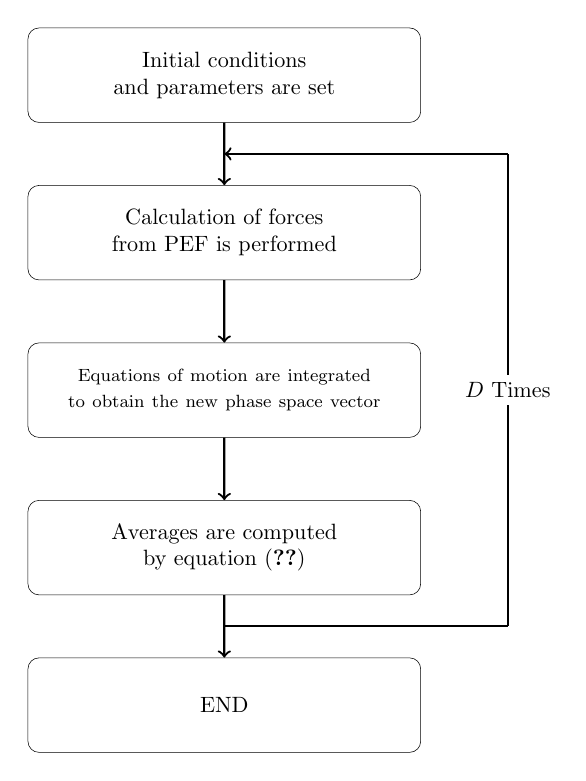
\begin{tikzpicture}[scale=0.8, transform shape]
	\node[rectangle,draw,rounded corners,very thin,minimum width=6cm,minimum height=1.5cm,text width=6cm,align=center] (A) at (0,10) {Initial conditions \\ and parameters are set};
	\node[rectangle,draw,rounded corners,very thin,minimum width=6cm,minimum height=1.5cm,text width=6cm,align=center] (B)  at (0,7.5) {Calculation of forces \\ from \ac{PEF} is performed};
	\node[rectangle,draw,rounded corners,very thin,minimum width=6cm,minimum height=1.5cm,text width=6cm,align=center] (C)  at (0,5) {\footnotesize Equations of motion are integrated to obtain the new phase space vector};
	\node[rectangle,draw,rounded corners,very thin,minimum width=6cm,minimum height=1.5cm,text width=6cm,align=center] (D)  at (0,2.5) {Averages are computed \\ by equation~(\ref{eq:MDTimeAve})};
	\node[rectangle,draw,rounded corners,very thin,minimum width=6cm,minimum height=1.5cm,text width=6cm,align=center] (E)  at (0,0) {END};
	\draw[thick,->] (A) -- (B);
	\draw[thick,->] (B) -- (C);
	\draw[thick,->] (C) -- (D);
	\draw[thick,->] (D) -- (E);
	\draw[thick,-] (0,1.25) -- (4.5,1.25);
	\draw[thick,-] (4.5,1.25) -- (4.5, 8.75) node[pos=0.5, fill=white] {$D$ Times};
	\draw[thick,->] (4.5, 8.75) -- (0, 8.75);
\end{tikzpicture}
\caption{Schematic representation of an \acs{MD} simulation.}
\label{fig:MDscheme}
\end{figure}

\subsection{Initial configuration}
Before an \ac{MD} simulation can be performed it is necessary to select an \textit{initial configuration}. Its choice can be nontrivial and it depends on the complexity of the system. Moreover, all successive simulations will depend on the initial configuration, so if it is wrong, maybe even the simulations will produce wrong results. Then, careful attention must be paid in setting up the initial configuration.

Setting up an initial configuration means to prepare an $N$--particle system and give all the particle positions and velocities, i.e. give all the $6N$ coordinates of the initial phase space vector $\vec x_0$. The initial velocities can be extracted randomly from the Maxwell--Boltzmann distribution function at a specific system's temperature
\begin{equation*}
	f(v_i) = \sqrt{\frac{m_i}{2\pi k_B T}}e^{-\left ( \frac{m_iv_i^2}{2k_B T}\right )}
\end{equation*}
moreover the random assignment algorithm have to rescale all the velocities such that the total system's momentum $\vec P = \sum_{k=1}^N m_k\vec v_k$ is zero, this is equivalent to a \ac{COM} motion removal. This is done because, in general, the total force acting on the system $\vec F = \sum_{k=1}^N \vec F_i$ is zero, then the \ac{COM} motion is constant and to avoid a constant drift of the system in space this can be removed. Of course this is a constraint on the system and it must be taken into account because it reduces the system \ac{DOF} by $3$.

\subsection{Periodic boundary conditions}
In all experiments our system is necessarily confined into a box with its initial size. Even in an \ac{MD} simulation the sample system is inserted into a \textit{simulation box} whose shape can be differently chosen to better reproduce the symmetry of the simulated system. That box gives us the trivial possibility to introduce a well defined reference system of coordinate in which respect the particles positions are assigned. Obviously we must not forget to correctly treat the \textit{boundary conditions}. In order to avoid surface effects and to consider only an infinite bulk system, \ac{PBC} are imposed to the simulation box. This gives us also the possibility to simulate system's bulk proprieties without considering a large number of particles.
\begin{SCfigure}
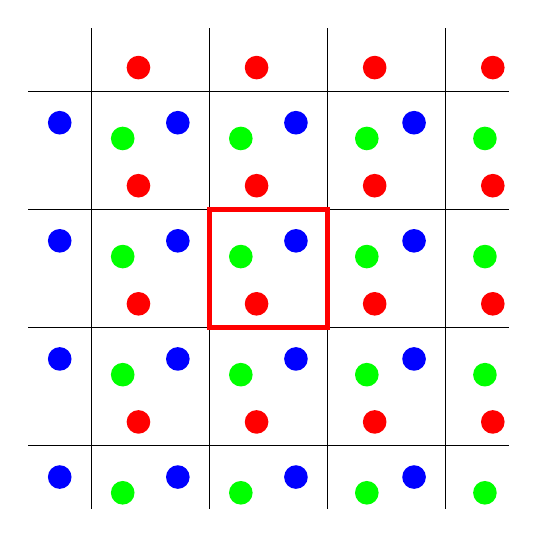
\begin{tikzpicture}
	\draw[step=1.5cm,thin] (-0.8,-0.8) grid (5.3,5.3);
	\draw[draw=red,ultra thick] (1.5,1.5) rectangle (3,3);
	\foreach \x in 	{0.6,2.1,3.6,5.1}
		\foreach \y in {0.3,1.8,3.3,4.8}
			\fill[fill=red] (\x,\y) circle (0.15);
	\foreach \x in 	{-0.4,1.1,2.6,4.1}
		\foreach \y in {-0.4,1.1,2.6,4.1}
			\fill[fill=blue] (\x,\y) circle (0.15);
	\foreach \x in 	{0.4,1.9,3.5,5}
		\foreach \y in {-0.6,0.9,2.4,3.9}
			\fill[fill=green] (\x,\y) circle (0.15);
\end{tikzpicture}
\caption{Schematic view of a two--dimensional box with \acs{PBC} imposed. The central, red contoured, box is the simulation box and it is replicated along each side.}
\label{fig:pbc}
\end{SCfigure}
To give a better idea, in figure~(\ref{fig:pbc}) an example of a two--dimensional box with \ac{PBC} is shown. The central red contoured box is the simulation box. The idea is to replicate that box in space along each side so that there are no surface particles nor walls in the central box. When a particle moves in the central box, all its images virtually move the same way in the copies of the box so that if a particle leaves the virtual boundary of the central box, then, its nearest image enters the box and the number density of particles in the simulation box is conserved.
This virtual movement of image particles is achieved adjusting the positions of the simulation box particles which have left the main box. For example, if one use a cubic box and a particle crosses its boundary in one direction, say the $x$ direction, then its coordinate is corrected by subtracting (if it leaves the box in the positive direction) or adding the box side length parallel to $x$ direction. Even if the most used shape is the cubic one, not all the shapes are accessible to impose the \ac{PBC}, the most useful example is a spherical shape. When it is possible one have to use the most appropriate shape to better describe the symmetry of the system, otherwise a closest approximation, compatible with \ac{PBC}, must be used.

Even if \ac{PBC} are used in a wide range of applications, it must be taken into account that imposing periodicity to a system may affect its properties. A clear limitation of the periodic cell is that it is not possible to achieve fluctuations that have a wavelength greater then the cell length. This cause, obviously, the impossibility to sample those vibrating modes. Another problem arises with the range of the inter--particles interactions: one have to choose carefully the size of the simulation box, or the number of particles if an $NPT$ ensemble is used, to ensure that the smallest simulation box length is greater then the interaction range. This can be made easily for example with the Van der Waals interaction. On the contrary it is a difficult and time consuming task to do the same with the electrostatic interaction that it treated with a more sophisticated methods (this will be better explained in section~\ref{sec:longRangeInt}).

\subsection{Numerical integrators}
As we have seen above we need to solve numerically the equations of motion. Since the \ac{PEF} is a continuous function of the phase space vector at a time $t$, the simplest way is to use the so called \textit{finite difference} method. The basic idea is to expand the Newton's law in a Taylor series as follow
\begin{equation}
	\vec r_i(t + \delta t) = \vec r_i(t) + \vec v_i(t)\ \delta t + \frac{1}{2m_i}\vec f_i(t)\ (\delta t)^2\ +\ o((\delta t)^3)
	\label{eq:newtonTaylor}
\end{equation}
where we used the identities $\vec v_i(t) = \dot{\vec r}_i(t)$ and $m_i\ddot{\vec r}_i(t) = \vec f_i(t)$.

From this point, different algorithms have been developed. In the following we will describe in detail the most important, the \textit{Verlet algorithm}, and its implementation the \textit{leap--frog algorithm}, which is the default used in our \ac{MD} tools for this thesis work.

\subsubsection{Verlet algorithm}
The Verlet algorithm requires the positions and the forces at a time $t$ and the positions at a time $t-\delta t$ to calculate the  positions at a time $t+\delta t$. Starting from equation~\eqref{eq:newtonTaylor} we can write
\begin{align}
	\vec r_i(t+\delta t) &\simeq \vec r_i(t) + \vec v_i(t)\delta t + \frac{1}{2m_i}\vec f_i(t)\ (\delta t)^2
	\label{eq:verlet1} \\
	\vec r_i(t-\delta t) &\simeq \vec r_i(t) - \vec v_i(t)\delta t + \frac{1}{2m_i}\vec f_i(t)\ (\delta t)^2
	\label{eq:verlet2}
\end{align}
from their sum we obtain the new positions at a time $t+\delta t$
\begin{equation*}
	\vec r_i(t+\delta t) \simeq 2 \vec r_i(t) - \vec r_i (t - \delta t) + \frac{1}{m_i}\vec f_i(t)\ (\delta t)^2
\end{equation*}
The velocities do not appear in the equation above and can be obtained taking the difference of equation~\eqref{eq:verlet1} and~\eqref{eq:verlet2}
\begin{equation*}
	\vec v_i(t) \simeq \frac{\vec r_i(t+\delta t) - \vec r_i(t-\delta t)}{2\delta t}
\end{equation*}
Since positions are computed as differences this is a fourth order algorithm and the precision is up to $o(\delta t)^4$, but they also contain a small term ($o(\delta t)^2$) which is summed to a difference of larger terms, this may cause a loss of precision.

The main disadvantage is that the velocities at a time $t$ are an output of the calculation and not a part of the algorithm itself; moreover it is not self--starting because the algorithm required the positions at a time $t-\delta t$. At $t=0$ we need a trick for obtain the previous inexistent positions. The trick is to use the equation~\eqref{eq:verlet2} truncated at the first order: $\vec r_i(-\delta t) \simeq \vec r(0) - \vec v_i(0)\delta t$.

\subsubsection{Leap--Frog algorithm}
The leap--frog algorithm is a variant of the Verlet one and it is commonly implemented in many \ac{MD} tools, as is our case. It computes the positions at a time $t$ and the velocities at a time $t+\nicefrac{\delta t}{2}$ from the forces at a time $t$ and the velocities at a time $t-\nicefrac{\delta t}{2}$. The main advantage with respect to the Verlet algorithm, is that it is self--starting because is does not require the positions at a time $t-\delta t$.

First it calculates the velocities at a time $t+\delta t/2$ as follow
\begin{equation*}
	\vec v_i(t + \nicefrac{1}{2}\delta t) \simeq \vec v_i(t - \nicefrac{1}{2}\delta t) + \vec a_i(t)\delta t
\end{equation*}
then the positions at a time $t+\delta t$ are computed
\begin{equation*}
	\vec r_i(t + \delta t) \simeq \vec r_i(t) + \vec v_i(t + \nicefrac{1}{2}\delta t)\delta t
\end{equation*}
The velocities at a time $t$ can be calculated by
\begin{equation}
	\vec v_i(t) \simeq \frac{\vec v_i(t + \nicefrac{1}{2}\delta t) + \vec v_i(t - \nicefrac{1}{2}\delta t)}{2}
	\label{eq:lfVelocitiesSync}
\end{equation}

Another advantage is that the velocities are part of the algorithm itself and moreover it does not require the calculation of the difference between two large numbers, with an increasing of precision. The obvious disadvantage is that the positions and velocities are not synchronized so the equation~\eqref{eq:lfVelocitiesSync} is necessary to calculate the velocities at a time $t$. The need to have velocities at the same time of positions, as for the Verlet algorithm, derives from the calculation of the kinetic energy contribution to the total energy: It must be computed with positions and velocities at the same time.
%Discorso energia cinetica nello stesso tempo delle posizioni

\subsection{Neighbor list}
\label{sec:neighbor}
In order to solve the classical equations of motion, it is necessary to know the forces, and so the \ac{PEF}, acting on the system's particles. As we shall see in detail in the next section, this is one of the most time consuming part of an \ac{MD} simulation. Even for a simple pairwise potential to known the forces acting on one particle, in principle, it is necessary to calculate the contribution from all particles in the simulation box and all other images. The most popular way to speed up the simulation is the use of a truncation of the interaction potentials within a cutoff. The general idea is to compute the interactions between those particles that are closer to the selected one by a certain cutoff distance $r_c$. By itself, the use of a truncation of the potential, may not dramatically reduce the time consuming in computing the inter--particles interactions.
This is because, in order to decide for what particles we have to compute the interactions, we have to compute the distances between every pair of particles in the system. A marked increase of the performance is achieved by the use of a \textit{neighbor pair--list}. The simplest way is to consider, for each particle, a list of its neighbor particles that lie within a sphere of radius $r_c$ surrounding the selected particle. Then, for each particle, the interactions are computed between the selected particle and those that are in its pair--list. There is a gain in performance if the pair--list is updated at least every $M>1$ \ac{MD} steps. This is possible because of the assumption that a particle neighbors do not change significantly for $M$ time steps, typically $M=10$ or $20$.

Anyway particles move during the non--updating time so that some of them may cross the pair--list causing an over-- or under--estimation of the inter--particles contribution. To partially solve this problem, as suggested by Verlet \cite{VerletList}, one can consider a \textit{buffered} pair--list or a \textit{Verlet cut--off scheme} in which the pair--list is constructed considering those particles that are close to the selected one by a distance of $r_l > r_c$, called \textit{list radius}. That pair--list is updated every some time steps, but every time steps the
pairwise contribution is computed only between those particles in the pair--list for which the distance is less then $r_c$. Thus, at the cost of slightly decrease the performance compared to the un--buffered pair--list, almost none of the interacting particles within the cutoff is neglected. Nevertheless, since a too big list radius and a too small list update frequency leads to a loss of performance, particle--pairs could still move enough during the non--update
time and have a chance to cross the boundary of the buffered pair--list $r_l$. This chance leads to a small energy drift proportional to the system temperature. In simulations with a constant temperature coupling i.e. in a canonical or isothermal--isobaric ensemble, the extra radius of the buffered pair--list can be dynamically determined, during the simulation, by fixing an upper limit to the energy drift. That tolerance is often called \textit{Verlet buffer tolerance} and commonly is set to $0.005$~kJ/(mol$\cdot$ps). In figure~(\ref{fig:pairlist}) a schematic representation of the buffered pair--list construction is shown.
\begin{SCfigure}
	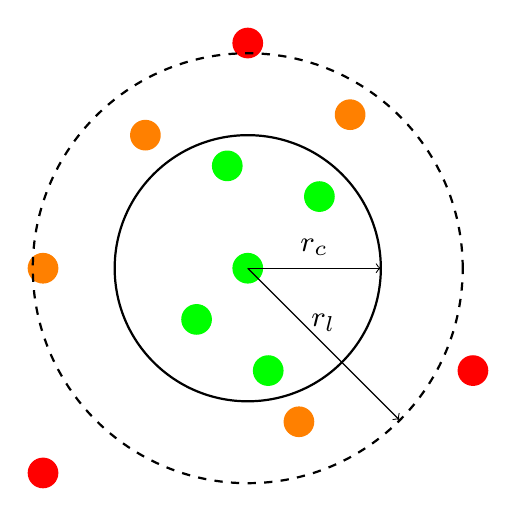
\begin{tikzpicture}[scale=1.3, transform shape]
		%\draw[gray,step=1] (-2,-2) grid (2,2);
		\fill[fill=green] (0,0) circle (0.15);
		\fill[fill=green] (-0.2,1) circle (0.15);
		\fill[fill=green] (-0.5,-0.5) circle (0.15);
		\fill[fill=green] (0.2,-1) circle (0.15);
		\fill[fill=green] (0.7,0.7) circle (0.15);
		\fill[fill=orange] (1,1.5) circle (0.15);
		\fill[fill=orange] (-1,1.3) circle (0.15);
		\fill[fill=orange] (-2,0) circle (0.15);
		\fill[fill=orange] (0.5,-1.5) circle (0.15);
		\fill[fill=red] (2.2,-1) circle (0.15);
		\fill[fill=red] (0,2.2) circle (0.15);
		\fill[fill=red] (-2,-2) circle (0.15);
		\draw[thick] (0,0) circle (1.3);
		\draw[dashed,thick] (0,0) circle (2.1);
		\draw[->] (0,0) -- (1.3,0) node[midway,above] {\footnotesize $r_c$};
		\draw[->] (0,0) -- (1.48, -1.48) node[midway,above] {\footnotesize $r_l$};
	\end{tikzpicture}
	\caption{Schematic representation of the buffered pair--list construction respect to the central particle.
	Green particles are in the pair--list below the cutoff radius $r_c$, therefore included in the calculation of the interactions. Orange particles are in the pair--list for which every step is checked if their distances became lower then $r_c$. Red particles are not in the pair--list thus are no more considered in the distance check, until the next list update.}
	\label{fig:pairlist}
\end{SCfigure}

A better performance can be achieved adding a dynamic update algorithm of the pair--list refresh rate during the simulation. A nice way is considering the maximum distances traveled by a particles in the pair--list: if this distance is greater than $r_b = r_l - r_c$ then the pair--list is certainly updated. From this one can fix the refresh rate to a higher value increasing the performance.

\subsection{Thermostat algorithms} %Molecular Modelling, 382
A thermostat is a external tool that allow us to maintain a system at a constant temperature. In \ac{MD} simulations if one want to use isothermal ensemble, so with constant temperature, some algorithms have to be developed in order to mimics the thermostat effect on the system and which generates the correct ensemble. One way to impose a constant temperature is acting on the particles velocities. A common practice, as suggested by Bussi \etal\, \cite{Bussi} is related to a \textit{velocity rescale} algorithm in which the velocities of all particles are scaled by some factor. The simplest way is to consider the total kinetic energy $K$ of the system as in equation~\eqref{eq:kinetic} and the average kinetic energy $\ave{K}$ obtained from equation~\eqref{eq:kineticT} with the substitution $3N\rightarrow N_f$
\begin{equation*}
	\ave{K} = \frac{1}{2}N_f k_B T
\end{equation*}
where $N_f$ is the \textit{total} \ac{DOF} of the system and $T$ is the target temperature. Thus the scaling factor is defined by
\begin{equation*}
	\alpha_{T} = \sqrt{\frac{\ave{K}}{K}}
\end{equation*}
The scaling operation is usually performed at a fixed rate during the simulation, or when the kinetic energy exceeds the limits of an interval centered around the target value. However the sampled ensemble is not explicitly known but, since in the thermodynamic limit the average properties do not depend on the ensemble chosen, even this very simple algorithm can be used to produce useful results. Despite this, for small systems or when the observables of interest are dependent on the fluctuations rather than on the averages or when other methods assume a canonical sampling, this method cannot be safely used.

In order to obtain the correct canonical sampling Bussi \etal\, modify the way to calculate $\alpha_T$ so as to enforce a canonical distribution for the kinetic energy. The new scaling factor is obtained from
\begin{equation*}
	\alpha_{T} = \sqrt{\frac{K_T}{K}}
\end{equation*}
where $K_T$ is extracted with a stochastic procedure from the equilibrium canonical distribution of the kinetic energy, given by
\begin{equation*}
	P(K_T)dK_T \propto K_T^{N_f/2-1}\ e^{-\beta K_T}\ dK_T
\end{equation*}
where $P(K_T)dK_T$ is probability that the system have a kinetic energy between $K_T$ and $K_T + dK_T$.

Since velocities are scaled only after some \ac{MD} steps this can cause a discontinuity in the particles velocities just before and after the scaling step. To avoid this problem, the authors suggest that the choice of $K_T$ can be based on the previous value of $K$ so as to obtain a smoother evolution. The procedure proposed by Bussi \etal\, consist by the following steps
\begin{itemize}
	\item Evolve the system for a single time step solving the equations of motion, so as to be in an $NVE$ ensemble;
	\item Calculate the total kinetic energy and evolve it for a single time step using an auxiliary continuous stochastic dynamics;
	\item Rescale the velocities by $\alpha_T$ so as to enforce this new value of the kinetic energy.
\end{itemize}
The authors have shown that an auxiliary dynamics for the kinetic energy of the form
\begin{equation*}
	dK = \frac{\ave{K} - K}{\tau_T}\ dt + 2 \sqrt{\frac{K\ave{K}}{N_f\tau_T}}\ dW
\end{equation*}
can do the job. Where $dW$ is a Wiener stochastic noise and $\tau_T$ is an arbitrary parameter which is related to the response time of the thermostat. In fact it reduces to the simple velocity rescale if $\tau_T\rightarrow 0$ and to an Hamiltonian dynamics (as an $NVE$ ensemble) if $\tau_T\rightarrow +\infty$. Until the system is at non--equilibrium the first determinist part is dominant an drives the system to equilibrium with a characteristic time $\tau_T$. Then the stochastic contribution sample the canonical distribution.
 

\subsection{Barostat algorithms} %Molecular Modelling, 382
As the thermostat maintain the system at a constant temperature $T$, a barostat is needed for maintain the system at a constant pressure $p$. To do this the system is coupled to a sort of piston so that changing the volume will adjust the pressure. Thus the system volume must allowed to fluctuate. 

\subsubsection{Berendsen algorithm}
The simplest way, as proposed by Berendsen, is a scaling of both particle coordinates and volume. The rate of change of pressure is given by
\begin{equation*}
	\frac{dp}{dt} = \frac{p_0 - p}{\tau_p}
\end{equation*}
where $p_0$ is the target pressure, $p$ is the instantaneous system pressure given by equation~\eqref{eq:pressure} and $\tau_p$ is a coupling constant related to the response time of the barostat. Thus if we consider a time step $\delta t$ then the volume scaling factor $\lambda$ is given by
\begin{equation*}
	\lambda = 1- k_T (p_0 - p) \frac{\delta t}{\tau_p}
\end{equation*}
where $k_t$ is the isothermal compressibility defined as
\begin{equation*}
	k_T = -\frac{1}{V}\left ( \frac{\partial V}{\partial p}\right )_{T}
\end{equation*}
while the factor $\nicefrac{\delta t}{\tau_p}$ give a scaling factor for the isothermal compressibility that allow us to take into account the finite response time of the barostat. If $\tau_p \rightarrow 0$ it is like the system has an infinity isothermal compressibility so it is necessary a really small change in volume to achieve the correct pressure; on the contrary if $\tau_p \rightarrow +\infty$ the system is reduced an Hamiltonian dynamics. The particle coordinates is scaled by the factor $\lambda^{\nicefrac{1}{3}}$. 

\subsubsection{Parrinello--Rahman algorithm}





